\documentclass[a4wide,12pt]{article}

\usepackage{verbatim}
\usepackage{listings}
\usepackage{graphicx}
\usepackage{a4wide}
\usepackage{color}
\usepackage{amsmath}
\usepackage{amssymb}
\usepackage[T1]{fontenc}
\usepackage{cite} % [2,3,4] --> [2--4]
\usepackage{shadow}
\usepackage{hyperref}
\usepackage{fancyhdr}

\pagestyle{fancy}
\fancyhead[CO,CE]{Lars Christian Hauge}
\begin{document}
\section*{Project 2}

\subsection*{Abstract}
In this project I have used Jacobi's algorithm to find the eigenvalues of a harmonic oscillator well with one and later two electrons.
I have looked at the efficiency of Jacobi's method by comparing it to armadillo's eigenvalue solver.
Lastly I found eigenvectors for the three lowest energy levels of the oscillator system and plotted them against the relative distance between the electrons. 

\subsection*{Introduction}
The aim for this project is to solve Schr\"odinger's equation for two electrons in a three-dimensional harmonic oscillator well. 
Doing this we get an eigenvalue problem that we are going to solve using Jacobi's method. We are first going to study just one electron in a harmonic oscillator well, to see how efficient and precise Jacobi's method is. 
I am going to compare it with armadillo's way of finding eigenvalues. Then I am going to put a new electron in the potential to see how this affects the system.

\subsection*{Methods}
The first thing I am asked to do is to write a function which implements Jacobi's rotation algorithm. 
Jacobi's rotation algorithm goes like this; if we have a symmetric matrix $\textbf{A}$ and a rotation matrix $\textbf{S}$.
Where the rotation matrix's elements that differ from zero are: $\textbf{S}_{kk} = \textbf{S}_{ll} = \cos\theta, \textbf{S}_{kl} = -\textbf{S}_{lk} = \sin\theta and \textbf{S}_{ii} = 1, i \neq k, l$.
Then $\textbf{B} = \textbf{S}^\intercal \textbf{A} \textbf{S}$ is symmetric and similar and has entries:

$\textbf{B}_{kk} = c^2\textbf{A}_{kk}-2cs\textbf{A}_{kl}+\textbf{A}_{ll}s^2$

$\textbf{B}_{ll} = c^2\textbf{A}_{ll}+2cs\textbf{A}_{kl}+\textbf{A}_{kk}s^2$

$\textbf{B}_{ik} = \textbf{A}_{ik}c - \textbf{A}_{il}s, i \neq k,l$

$\textbf{B}_{il} = \textbf{A}_{il}c + \textbf{A}_{ik}s, i \neq k,l$

$\textbf{B}_{kl} = (\textbf{A}_{kk}-\textbf{A}_{ll})cs + \textbf{A}_{kl}(c^2 - s^2)$

where $c = \cos\theta$ and $s = \sin\theta$. 

We want to choose $\theta$ so that all non-diagonal elements $\textbf{B}_{kl} = \textbf{B}_{lk} = 0$.
This gives $(\textbf{A}_{kk}-\textbf{A}_{ll})cs + \textbf{A}_{kl}(c^2 - s^2) = 0$ and after some algebra we have:
\[
\cot{2\theta} = \tau = \frac{\textbf{A}_{ll} - \textbf{A}_{kk}}{2\textbf{A}_{kl}}
\]
and after using $\cot{2\theta} = frac{1}{2}(\cot\theta - \tan\theta$ we end up with the quadratic equation
\[
t^2 + 2\tau t - 1 = 0
\]
which gives 
\[
t = \tan\theta = - \tau \pm \sqrt{1+\tau^2}. 
\]

$C$ and $s$ I obtain by $c = {1}{\sqrt{1+t^2}}$ and $s = ct$. 
Now we have Jacobi's method, it is just to repeat this many times till all non-diagonal elements are essentially zero, and we will eventually get the eigenvalues in the diagonal.
Here is how I have implemented Jacobi's method in c++. 
First we have the main part that loops through the functions.
\lstinputlisting[language=c++, firstline=29, lastline=40]{project2.cpp}
Then we have the part that does the actual work and rotates the matrix, and find the new entries to our matrix.
\lstinputlisting[language=c++, firstline=9, lastline=49]{Jacobi_rotate.hpp}
Lastly we have the part that searches after the largest non-diagonal element in the matrix so we can rotate around that. 
\lstinputlisting[language=c++, firstline=9, lastline=23]{offdiag.hpp}
It could also be interesting to see how I made my matrix for in the last part.
\lstinputlisting[language=c++, firstline=18, lastline=28]{project2c.cpp}

To find eigenvalues to compare with to see if I have found the right ones, I used the armadillo function $\textit{eig\_sym}$. I also used this to find the eigenvectors in the last exercise.
When I first tried this for $n = 100$ and $\rho_{max} = 1$ , I could not get the right eigenvalues(3, 7, 11...). It was not until I changed $\rho_{max}$ to 4.5 that I began to get real precision for the eigenvalues.
As  $\rho_{max}$ is supposed to be about infinite it is somewhat unfortunate that the step size changes when $\rho_{max}$ is changed. I think I have found a nice value that is not too low. 

\subsection*{Results}
We are asked in the text why we should choose $t = \tan\theta = -\tau\pm\sqrt{1+\tau^2}$ to be the smaller of the roots. By choosing the smaller of the roots we make sure that $|\tan\theta| \leq 1$ which again makes $|\theta| \leq \frac{\pi}{4}$. 
This again makes sure that $c$ becomes as large as possible which minimizes 
\[
||{\bf B}-{\bf A}||_F^2=4(1-c)\sum_{i=1,i\ne k,l}^n(a_{ik}^2+a_{il}^2) +\frac{2a_{kl}^2}{c^2}.
\]
and makes sure that each step in the Jacobi's method gets you closer to a diagonal matrix and the eigenvalues instead of setting you back.

I never got all eigenvalues with four leading digits for the same n, with $n = 100$ and $\rho_{max} = 4.5$ I got 2.99938, 6.99702 and 10.9981 as the three lowest eigenvalues. 
I got the exact same thing with the armadillo function and the Jacobi rotation I implemented myself, what confused me after testing the program was that for higher n(=200) the precision went down for the third eigenvalue, but increased for the two lowest. 
It was the exact same thing for the armadillo function so I assume it is the initial matrix that is not so precise.

You needed many similarity transformations before all non-diagonal elements became essentially zero. We see that we need just over $n^2$ transformations 
before we get a nice matrix. 

\begin{tabular}{|c|c|c|}
\hline
	n & nr. of transf. &  \\ \hline
	10 & 161 & 1.6$n^2$ \\ \hline
	50 & 4329 & 1.7$n^2$ \\ \hline
	100 & 18439 & 1.8$n^2$ \\ \hline
	200 & 71624 & 1.8$n^2$ \\ \hline
\end{tabular}

When comparing time usage I found, not surprisingly, that the armadillo function was much faster than Jacobi's method. I found the time usage for n=100 and n=200.

\begin{tabular}{|c|c|c|}
\hline
	n & Jacobi & armadillo \\ \hline
	100 & 1.313s & 0.020s \\ \hline
	200 & 19.172s & 0.073s \\ \hline
\end{tabular}

When I added another electron I did not know what the eigenvalues should be, so I checked against Taut's article with oscillator frequency $\omega_r = 0.05$. My program did not give anything similar to what he got
no matter how I chose the $\rho_{max}$. In the end I just went for $\rho_{max} = 5.0$ and n = 100, because I could not find a fault. 
The eigenvalue for the lowest energy state was:

\begin{tabular}{|c|c|}
\hline
	$\omega_r$ & $\epsilon_0$ \\ \hline
	0.01 & 0.84 \\ \hline
	0.5 & 2.23 \\ \hline
	1.0 & 4.06 \\ \hline
	5.0 & 17.43 \\ \hline
\end{tabular}

We see that the energy increases with higher oscillator frequency just as in the article to Taut, which must mean I have done something right. 

Lastly I have generated a number of plots that shows the wave function for different frequencies and energies. I have included both the square of the wave function and the wave function alone for some cases and 
have also for all energy levels plotted with and without the repulsion between the electrons. All the plots are collected on the last two pages of this report.
\begin{figure}[p]
	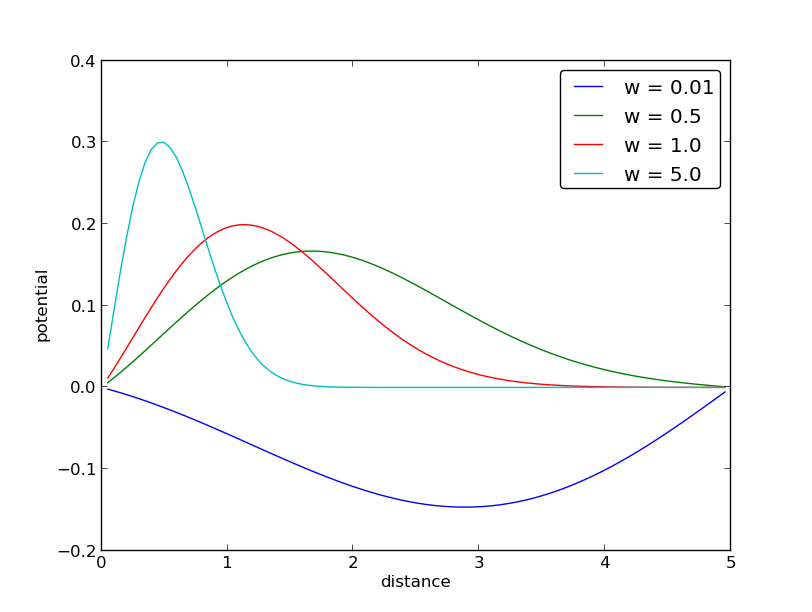
\includegraphics[width=80mm]{electronpotential}
	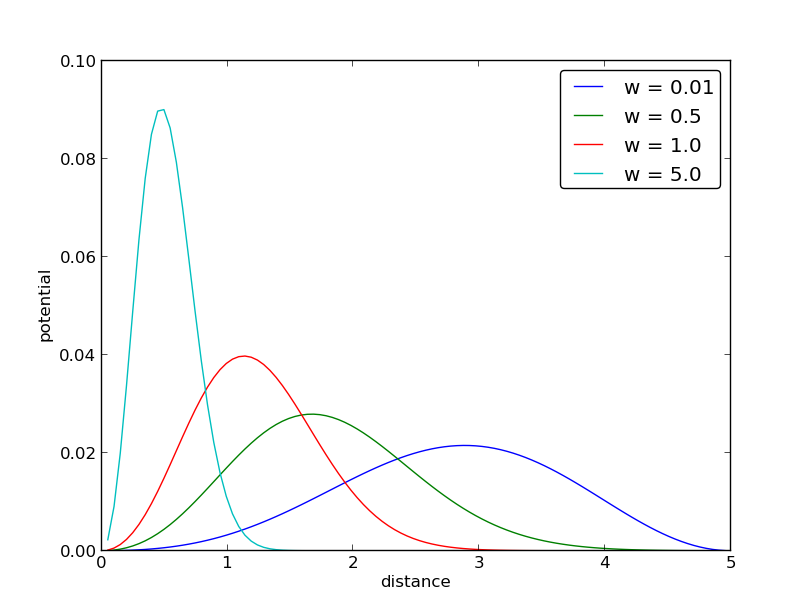
\includegraphics[width=80mm]{electronpotentialsquare}
		\caption{Ground state of the well, the one to the right is the square of the other}
\end{figure}
\begin{figure}[p]
	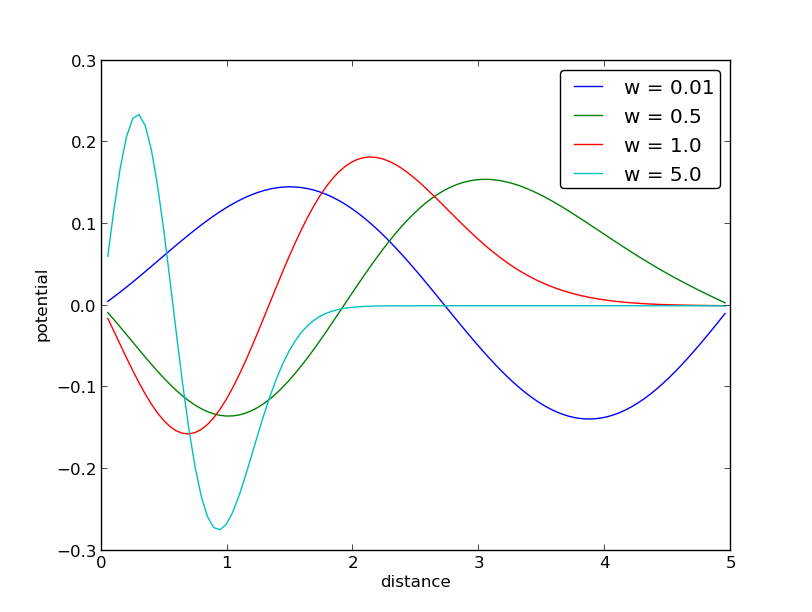
\includegraphics[width=80mm]{electronpotentialexc1}
	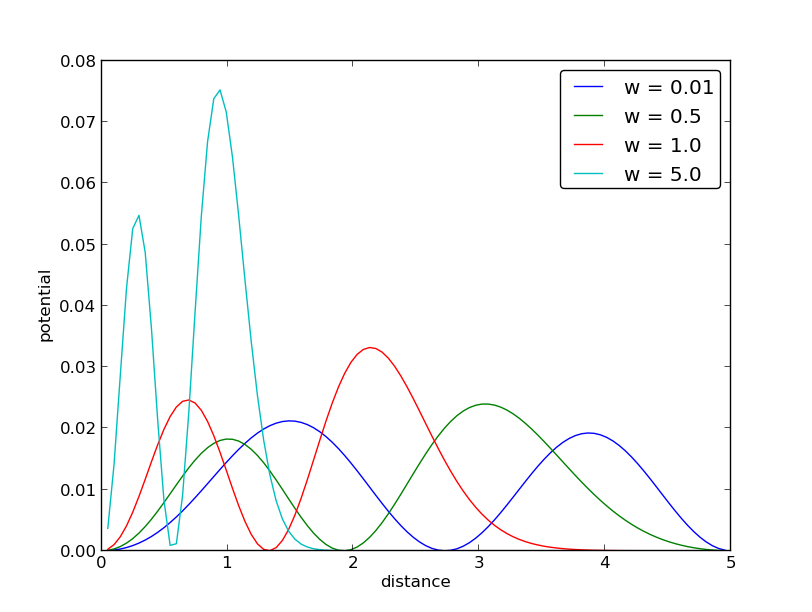
\includegraphics[width=80mm]{electronpotentialexc1square}
		\caption{First excited state of the well, the one to the right is the square of the other}
\end{figure}
\begin{figure}[p]
	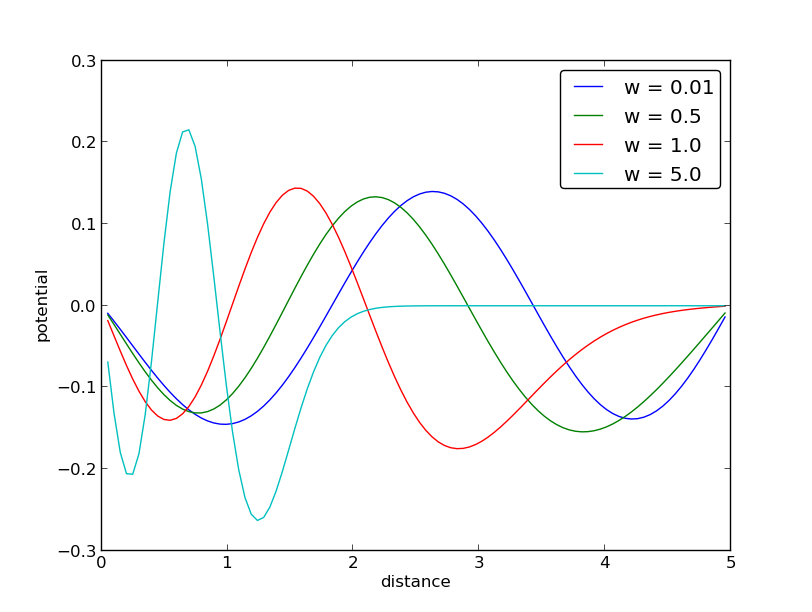
\includegraphics[width=80mm]{electronpotentialexc2}
	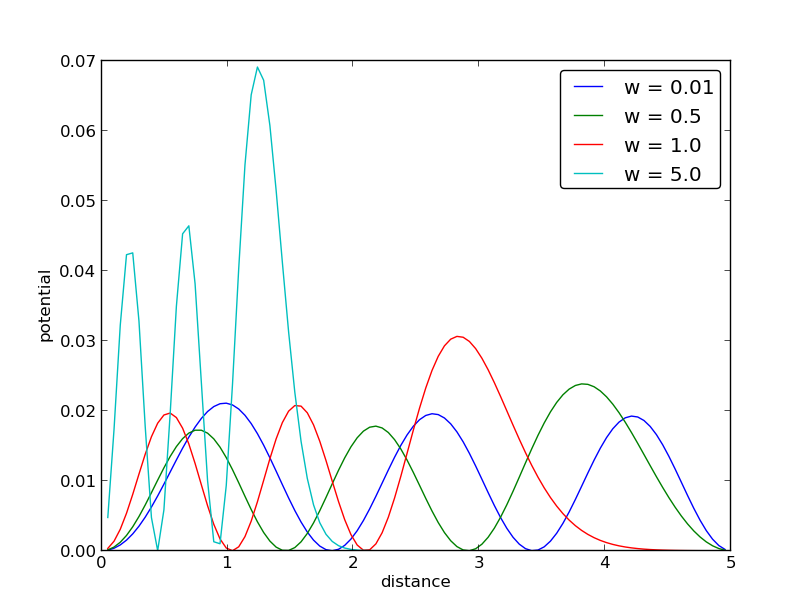
\includegraphics[width=80mm]{electronpotentialexc2square}
		\caption{Second excited state of the well, the one to the right is the square of the other}
\end{figure}	 
\begin{figure}[p]
	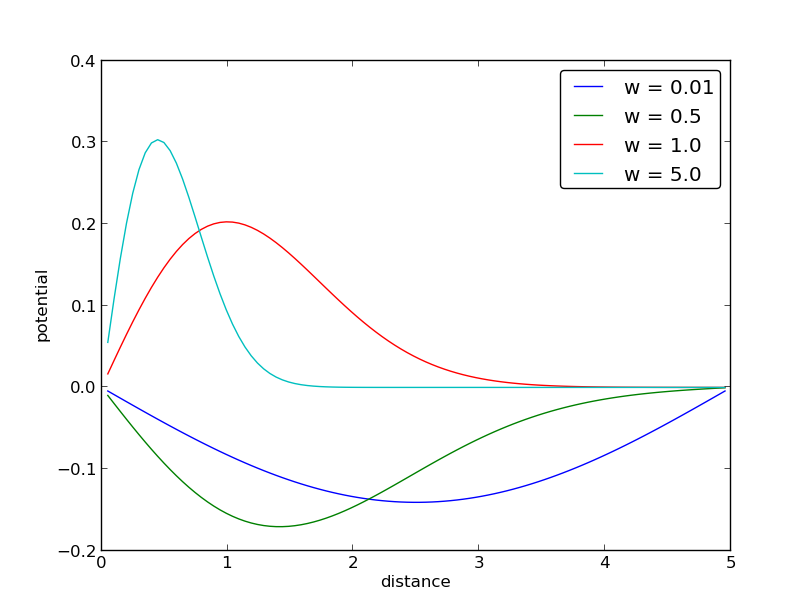
\includegraphics[width=70mm]{potential}
	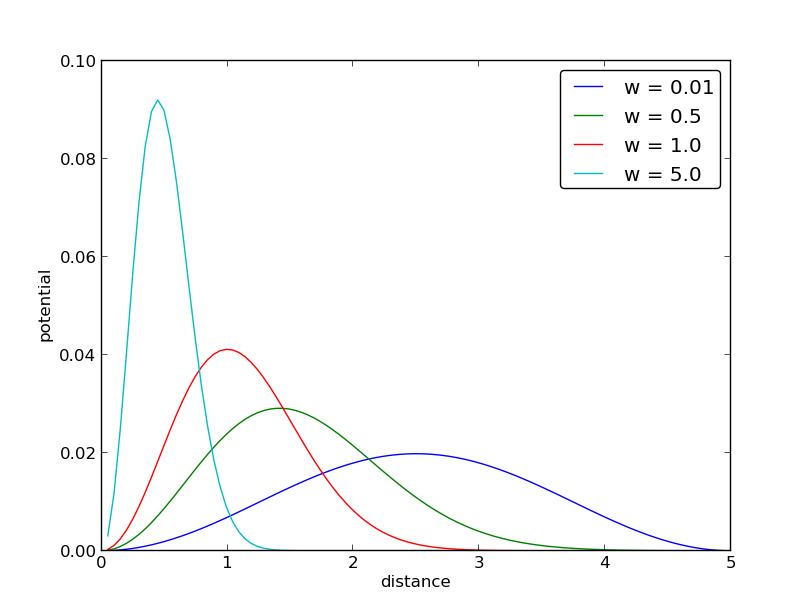
\includegraphics[width=70mm]{potentialsquare}
		\caption{Ground state of the well without electron repulsion, the one to the right is the square of the other}
\end{figure}	 
\begin{figure}[p]
	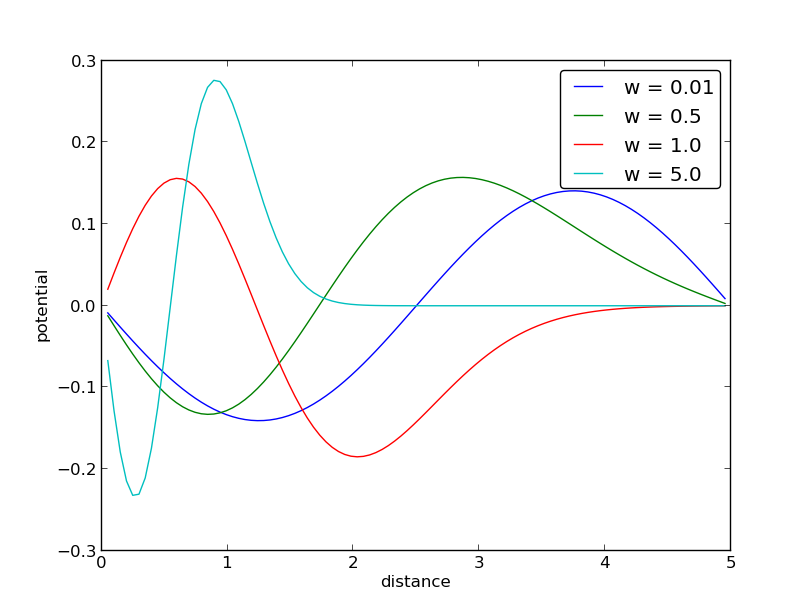
\includegraphics[width=70mm]{potentialexc1}
	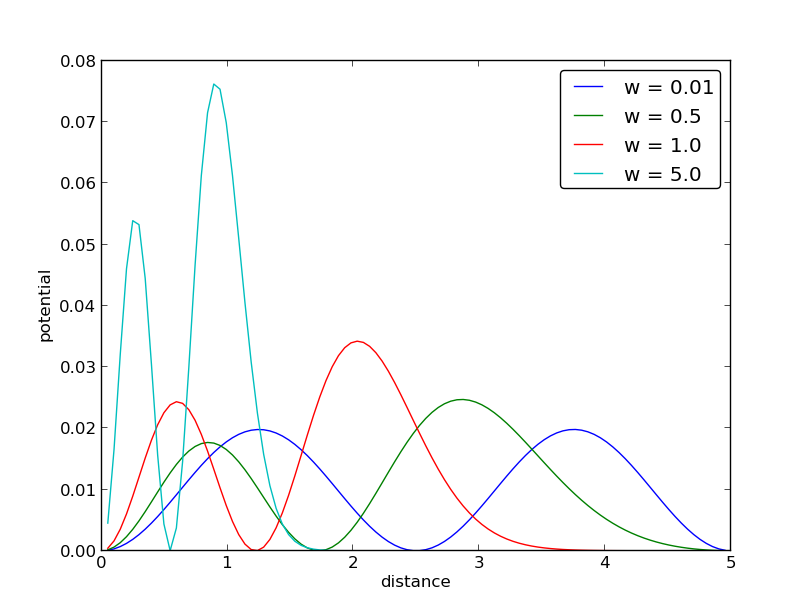
\includegraphics[width=70mm]{potentialexc1square}
		\caption{First excited state of the well without electron repulsion, the one to the right is the square of the other}
\end{figure}	
\begin{figure}[p]
	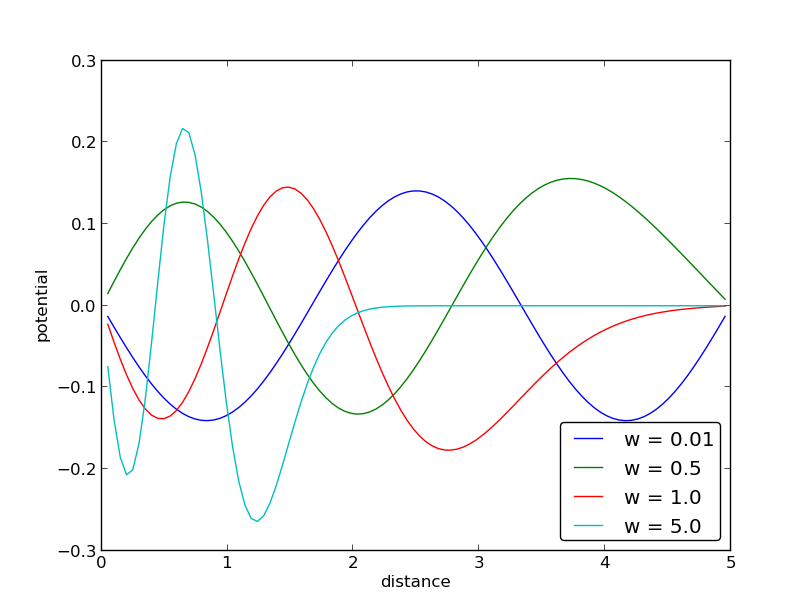
\includegraphics[width=70mm]{potentialexc2}
	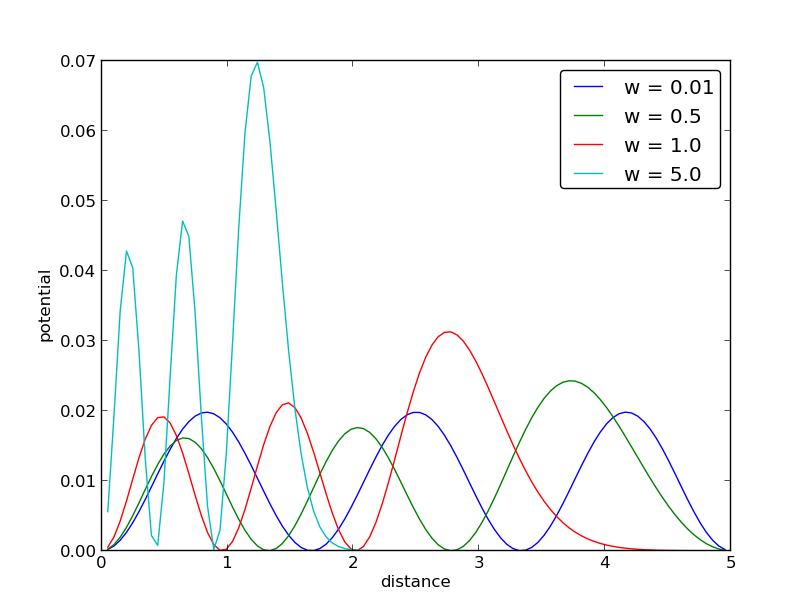
\includegraphics[width=70mm]{potentialexc2square}
		\caption{Second excited state of the well without electron repulsion, the one to the right is the square of the other}
\end{figure} 

We see that it is mainly for $\omega_r = 0.5$ that we have any difference for the electron repulsion. We see that without the electron repulsion it becomes the inverse of the graph with repulsion.


\subsection*{Conclusion}
In this exercise we have seen that Jacobi's method is not very fast as an eigenvalue method compared to armadillo's method for finding eigenvalues. They are about equally precise, so there are faster algorithms which gives the same result faster. Unfortunately
they are harder to implement, so choosing Jacobi's method is not that idiotic. 

We have seen how we can solve a harmonic oscillator problem numerically and seen how its energies behaves when putting in electrons for different oscillator frequencies. 


\end{document}